\chapter{Автоматическое планирование}

\section{Интеллектуальный агент. Проблемная среда}

Под \emph{интеллектуальным агентом} понимают сущность, действующую в некоторой проблемной среде, получая информацию о ней с помощью сенсоров и воздействуя через исполнительные механизмы. Введем классификацию таких сущностей в форме PEAS:

\begin{itemize*}
\item
  Performance -- \emph{критерии производительности}, которые стремиться
  максимизировать агент
\item
  Environment -- \emph{описание окружающей среды}, предметной области\footnote{Здесь и далее понятия проблемная, окружающая среда, предметная область и система будем считать взаимозаменяемыми.}
\item
  Actuators -- \emph{исполнительные механизмы}, или действия
\item
  Sensors -- доступные агенту \emph{датчики}
\end{itemize*}

Термином \emph{восприятие} обозначаются полученные агентом сенсорные
данные в любой конкретный момент времени.

\emph{Последовательностью актов восприятия} агента называется полная
история всего, что было когда-либо им воспринято.

\emph{Рациональный агент} для каждой возможной последовательности актов восприятия
 должен выбрать действие, которое, как ожидается, максимизирует его показатели производительности, с учетом фактов, предоставленных данной последовательностью актов восприятия и всех встроенных знаний, которыми обладает агент.
 
Проблемная среда сама по себе также может быть охарактеризована с помощью ряда признаков:

\begin{description}
\item[Полностью или частично наблюдаемая] \hfill \\
  Среда называется полностью  наблюдаемой, если датчики агента предоставляют ему доступ к полной
  информации о состоянии среды в каждый момент времени. Частичная
  наблюдаемость может возникнуть, например, из-за создающих шум или
  неточных датчиков или из-за того, что отдельные характеристики ее
  состояния отсутствуют в информации, получаемой от датчиков.
\item[Детерминированная или стохастическая] \hfill \\Если следующее состояние среды
  полностью определяется текущим состоянием и действием, выполненным
  агентом, то такая среда называется детерминированной. В противном
  случае она является стохастической. Может создаться впечатление, что
  среда стохастическая в случае, когда она является частично
  наблюдаемой.
\item[Эпизодическая или последовательная] \hfill \\В эпизодической среде опыт агента
  состоит из неразрывных эпизодов. Каждый эпизод включает в себя
  восприятие среды агентом, а затем выполнение одного действия. При этом
  каждый следующий эпизод не зависит от действий,\\предпринятых в
  предыдущих. В противоположность этому, в последовательных вариантах
  среды каждое текущее решение может повлиять на все будущие.
\item[Статическая или динамическая] \hfill \\Если среда может измениться в ходе того,
  как агент выбирает очередное действие, то такая среда называется
  динамической для данного агента, в противном случае -- статической.
\item[Дискретная или непрерывная] \hfill \\Различия между дискретными и непрерывными
  средами относятся к описанию состояния, способу учета времени,
  восприятиям и действиям агента.
\item[Одноагентная или мультиагентная] \hfill \\Иногда целесообразно рассматривать
  пользователя как второго агента.
\end{description}
 
Поведение агента определяется его программой. Далее в этой главе будет рассматриваться класс планирующих целенаправленных агентов. Их можно описать следущим образом: при заданных описаниях начального и целевого состояний среды, построить последовательность доступных действий, которая переводит среду из начального состояния в целевое.

Описываемые ниже подходы решают так называемую задачу полного планирования, когда план по достижению цели строится один раз и целиком. Это накладывает определенные ограничения на типы среды. Предполагается, что она является полностью наблюдаемой, детерменированной, последовательной, статической, дискретной, одноагентной.

\section{Классические алгоритмы планирования}

\subsection{Прямой и обратный вывод}

В случае, если состояние системы описано полностью и не совпадает ни с каким другим, назовем его 
\emph{физическим состоянием}. В таком случае исполнительные механизмы, или действия агента, будут представлять собой дуги направленного графа, где множество вершин будет совпадать с пространством всех возможных физических состояний среды.

Рассмотрим два классических подхода, являющихся разновидностями поиска в пространстве состояний. Особенностью этих алгоритмов является большой размер графа состояний. Пусть физическое состояние среды описывается набором из $N$ бинарных признаков. Тогда общее число физических состояний среды равно:

\begin{equation}
 S= \{ S_j: \langle A_1, \dots A_N \rangle, A_i \in \{0, 1\} \} \implies |S| = 2^N.
\end{equation}

На практике при использовании только бинарных признаков для описания их число может достигать нескольких сотен. Очевидно, что построить полный граф физических состояний не представляется возможным. Вводится понятие \emph{неявного графа}, вершины и ребра которого не имеют физического представления, а генерируются алгоритмически.

Как правило, описания доступных действий разделяются на пред- и постусловия, заданные на языке формальной логики\footnote{Далее будет использоваться язык пропозициональной логики для записи логических формул. Приложение 1 содержит его описание}. Таким образом, действие может быть выполнено тогда, когда выполняется его предусловие, а результатом выполнения будет физическое состояние, полученное путем применения постусловия к текущему состоянию.

Прямой логический вывод осуществляет попытку рекурсивно построить цепочку логических высказываний, соответствующую определенным пред- и постусловиям действий, которая приведет из старта в финиш.

В противоположность ему, обратный логический вывод решает аналогичную задачу, но в качестве начальной вершины выбирается целевое состояние.

\subsection{Сведение к задаче CSP (SAT)}

Другим подходом к решению задачи планирования является сведение к задаче CSP\footnote{CSP -- (англ. Constraint satisfaction problem) задача удовлетворения ограничений. }. При этом необходимо построить логическую формулу, которая выполнима тогда и только тогда, когда выполним план.

Неформально алгоритм построения формулы можно описать следующим образом. Пусть план содержит $k$ действий. Для каждого возможного действия $a$ введем булеву переменную:

\begin{equation}
 Action(a, i) = true \iff \text{действие a используется на шаге i}
\end{equation}

Для каждого бинарного признака в описании физического состояния также введем булеву переменную:

\begin{equation}
 Proposition(p, i) = true \iff \text{Признак p истинен на шаге i}
\end{equation}

Кроме того, вводятся дополнительные ограничения:
\begin{itemize}
 \item На каждом шаге может быть выполнено только одно действие (XOR-ограничения)
 \item Ограничения, описывающие постусловия действий
 \item Ограничения, описывающие неизменность признака, если он не был изменен действием
 \item Признак истинен на определенном шаге только как результат постусловия какого-либо действия
 \item Ограничения, описывающие начальное и конечное состояния
\end{itemize}

\subsection{Graphplan}

Также возможен подход с использованием специально сконструированного графа, обладающего следующими свойствами:

\begin{itemize}
 \item Направленный многоуровневый граф, где уровни чередуются
 \item Нечетные уровни (уровни состояний) представляют собой признаки, которые возможно являются положительными на $i$-м шаге плана.
 \item Четные уровни (уровни действий) представляют возможные действия, которые могли бы быть произведены на каждом шаге, включая бездействие.
 \item Дуги графа представляют собой пред- и постусловия
\end{itemize}

Построение графа происходит по правилам:

\begin{enumerate}
 \item Добавить действие на уровень $A_i$, если все его предусловия выполнены на уровне $S_i$
 \item Добавить литерал на уровень $S_i$, если он истинен в результате эффекта хотя бы одного действия на уровне $A_{i-1}$
 \item Уровень $S_0$ содержит все литералы из начального состояния
\end{enumerate}

\autoref{fig:graphplanimg} содержит пример построенного графа для одной из задач планирования.

\begin{figure}[H]
 \centering
 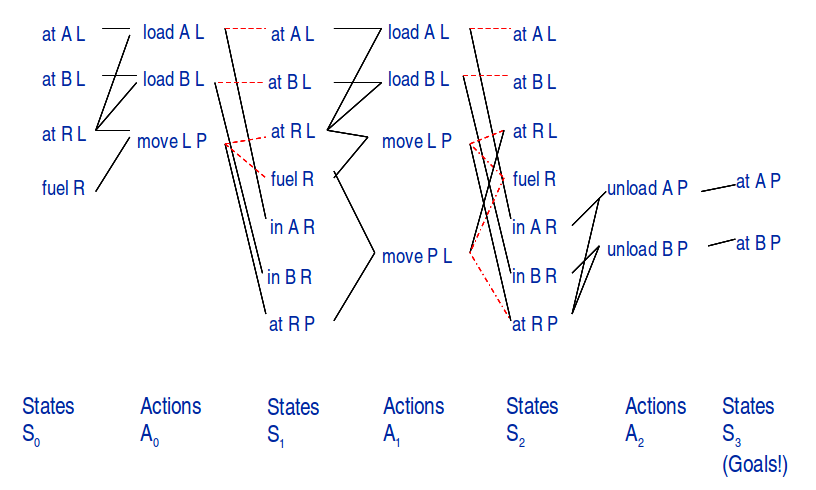
\includegraphics[width=1.0\textwidth]{c17_graphplan_satplan.png}
 \caption{Пример работы алгоритма Graphplan}
 \label{fig:graphplanimg}
\end{figure}

\section{Планирование в условиях частичной наблюдаемости}

Ранее предполагалось, что в любой момент времени агенту полностью известно текущее физическое состояние среды. Как правило, это не так. В этом разделе даются определения, необходимые для описания программ агентов, действующих в среде с частичной наблюдаемостью, и приводится одна из возможных стратегий -- условное планирование. Попутно вводится описания языка PDDL, являющегося академическим стандартом для описания проблем планирования.

\subsection{Пропозициональная логика}

При обсуждении условного планирования используется язык \emph{пропозицио\-нальной логики} (лат. propositio --- «высказывание»). Это раздел символической логики,
изучающий сложные высказывания, образованные из простых, и их
взаимоотношения. С точки зрения выразительности, логику высказываний
можно охарактеризовать как классическую логику нулевого порядка.

\subsubsection{Язык}

Алфавит языка разделен на три группы.

\begin{itemize*}
\item
  Пропозициональные переменные: $A, B, C, ...; A \in \{0, 1\}$;
\item
  Логические союзы: : $\neg$ --- знак отрицания, $\land$ --- знак
  конъюнкции, $\lor$ --- знак дизъюнкции, $\implies$ --- знак
  импликации, $\iff$ --- знак эквивалентности;
\item
  технические знаки: ( --- левая скобка, ) --- правая скобка.
\end{itemize*}

Сам язык можно индуктивно определить следующим образом:
\begin{enumerate}
 \item пропозициональная переменная есть формула;
 \item если $A$ -- произвольная формула, то $\neg A$ -- тоже формула;
 \item если $A$ и $B$ -- произвольные формулы, то $(A \implies B)$, $(A \land B)$, $(A \iff B)$, $(A \lor B)$ -- также формулы
\end{enumerate}

\subsubsection{Выполнимость булевых формул}

При работе с высказываниями пропозициональной логики возникает
\emph{задача выполнимости булевых формул}, SAT\footnote{SAT -- англ. boolean SATisfability problem}, которая формулируется так:
можно ли назначить всем переменным, встречающимся в формуле, значения
ложь и истина так, чтобы формула стала истинной. Известно, что эта
задача в общем случае обладает свойством $NP$-полноты.

\subsection{Язык PDDL}

Стандартом де-факто для описания задач планирования является язык
PDDL\footnote{Planning Domain Definition Language}. Основными его понятиями являются проблемная среда и задача (проблема), поставленная на ней в виде начального и конечного состояний. В дальнейшем понятия проблемная среда и предметная область будут рассматриваться как взаимозаменяемые.

В описании проблемной среды положим, что ее состояние задано набором
признаков. Для простоты будем все признаки полагать бинарными. Каждый
возможный набор их значений называется физическим состоянием среды.
Далее, представим датчики агента как акты восприятия значений одного или
более признаков. Исполнительные механизмы будут представлять собой
действия, переводящие среду из одного физического состояния в другое.

Проблемной среде исоответствуют следующая конструкция языка:

\begin{verbatim}
(define (domain <name>)
    <description>
)
\end{verbatim}

\subsection{Пример: мир Лампы}

Для более наглядного обсуждения планирующих агентов введем ``игрушечную'' проблему, которую неформально можно описать следующим образом: в некой
комнате находится лампа накаливания, соединенная выключателем с
источником питания. Там же находятся кондиционер и окно (считаем, что на
улице ночь). Необходимо включить свет.

\subsection{Доверительное состояние}

Более формально, введем набор бинарных признаков, описывающих среду:

\begin{itemize}
\item
  $L$. Свет горит (не горит)
\item
  $B$. Лампа исправна (неисправна)
\item
  $S$. Выключатель включен (выключен)
\item
  $W$. Окно открыто (закрыто)
\item
  $C$. Кондиционер включен (выключен)
\end{itemize}

Тогда например, состояние среды в котором лампа исправна, выключатель
выключен и свет не горит, представляет собой четыре различных физических
состояния:

\begin{equation}\langle \neg L, B, \neg S, \neg W, \neg C\rangle, \langle \neg L, B, \neg S, \neg W, C\rangle, \langle \neg L, B, \neg S, W, \neg C\rangle, \langle \neg L, B, \neg S, W, C\rangle,\end{equation}

Они получены перебором различных значений последних двух признаков.
Введем понятие доверительного состояния среды как подмножества множества
ее физических состояний. Для записи признаков, чье значение неизвестно,
введем сокращенную запись

\begin{equation}A?=A \lor \neg A\end{equation}

Тогда запись выше можно сократить до:

\begin{equation}\langle \neg L, B, \neg S, W?, C?\rangle\end{equation}

В PDDL для описания признаков используется следующая конструкция:

\begin{verbatim}
(: predicates (L) (S) (B) (W) (C) )
\end{verbatim}

Формализуем также описание задачи, задав начальное и конечное состояние
в виде логических формул:

\begin{verbatim}
(define (problem <name>)
    (: domain <domain_name> )
    (: init (~L) )
    (: goal (L) )
)
\end{verbatim}

\subsection{Действия}

Далее, введем действия, позволяющие изменять значения признаков.
Понятно, что в реальной среде не каждое действие доступно для выполнения
в любой момент времени. Поэтому вводятся понятия \emph{предусловия}(precondition) и
\emph{постусловия}(effect) действия как логических выражений с переменными в
множестве признаков. Если текущее физическое состояние не совпадает с
предусловием действия, то и его постусловие не будет выполнено.

\begin{table}[h]
\begin{tabular}{l | l | l | p{4cm} }
\hline
Действие & Описание & Предусловие & Постусловие \\
\hline
$chbulb$ & Заменить лампу & Выключатель выключен & Лампа исправна \\
\hline
$brbulb$ & Разбить лампу & Лампа исправна & Лампа неисправна. Свет не
горит \\
\hline
$onlight$ & Включить выключатель & Нет & Выключатель включен. Если лампа
исправна, свет горит \\
\hline
$offlight$ & Выключить выключатель & Выключатель включен & Выключатель
выключен. Свет не горит \\
\hline
$onwind$ & Открыть окно & Окно закрыто & Окно открыто \\
\hline
$offwind$ & Закрыть окно & Окно открыто & Окно закрыто \\
\hline
$oncond$ & Включить кондиционер & Кондиционер выключен & Кондиционер
включен \\
\hline
$offcond$ & Выключить кондиционер & Кондиционер включен & Кондиционер
выключен \\
\hline
\end{tabular}
\caption{Описание действий доступных в мире Лампы}
\end{table}

В PDDL действия содержатся в описании предметной области и задаются
следующей конструкцией:

\begin{verbatim}
    (: action ch_bulb ;Заменить лампу
        :precondition (B? & ~S)
        :effect (B)
    )
\end{verbatim}

Для заданного доверительного состояния выполнимость предусловия
какого-либо действия может быть неизвестной. Например, в состоянии
$\langle\neg L, B?, S?\rangle$ результатом действия $chbulb$ может оказаться как то же самое состояние
в случае, когда $S$ положителен, так и состояние
$\langle\neg L, B, \neg S\rangle$, когда предикат отрицателен.

\subsection{Аксиомы}

Можно заметить, что описания действий содержат дублирующуюся информацию.
Язык PDDL содержит понятие аксиомы - логической формулы, справедливой в
любом доверительном состоянии. Для мира Лампы справедлива следующая
аксиома: свет горит тогда и только тогда, когда лампа исправна и
выключатель включен.

\begin{equation} L \iff B \land S \end{equation}

Ей соответствует конструкция языка:

\begin{verbatim}
(: axiom (L <-> B & S) )
\end{verbatim}

\nameref{sec:appendix_problems} содержит полный вариант PDDL-описания мира Лампы.

\subsection{План -- граф доверительных состояний}

Так как мы рассматриваем частично наблюдаемые среды, то будем считать,
что агенту недоступно восприятие значений каких-либо признаков напрямую.
Результатом работы планировщика будет граф, отображающий возможные пути
из начального доверительного состояния в целевое. Классическим способом
представления неопределенности результата действия, рассмотренного
ранее, является $AND$-$OR$ граф.

\begin{algorithm}
  \caption{Алгоритм построения AND-OR графа}
  \begin{algorithmic}
   \Function{AndOrGraphSearch}{problem}
    \State \Return \Call{OrSearch}{Init, problem}
   \EndFunction
   \Function{OrSearch}{state, problem, path}
    \If{\Call{IsGoal}{problem, state}} \State \Return $\emptyset$ \EndIf
    \If{state $\in$ path} \State \Return Failure \EndIf
    \For{$(action, states)$ $\leftarrow$ \Call{Successors}{problem, state}}
    \State plan$\gets$ \Call{AndSearch}{states, problem, $state path$}
    \If{$plan \ne Failure$} \State \Return $[action \textbar plan]$ \EndIf
    \EndFor
    \State \Return Failure
   \EndFunction
   \Function{AndSearch}{states, problem, path}
    \For{$s_i \leftarrow states$}
      \State $plan_i \gets$ \Call{OrSearch}{$s_i$, problem, path}
      \If{$plan_i = Failure$} \State \Return Failure \EndIf
    \EndFor
    \State \Return $[$ \If{$s_1$} $plan_1 \dots$  \ElsIf{$s_{n-1}$} $plan_{n-1}$ \Else $plan_n$ \EndIf $]$
   \EndFunction
  \end{algorithmic}
\end{algorithm}

\autoref{fig:andorbulb} содержит пример построенного $AND-OR$ графа для мира Лампы.

\begin{figure}[H]
 \centering

 \begin{tikzpicture}[->,>=stealth', main node/.style={rectangle, draw}, l2 node/.style={circle, draw, minimum size=0.75cm},auto,node distance=3cm]
  \node[main node] (1) {$\neg L, B?, S?$};
  \node[l2 node] (2) [below left of=1] {};
  \node[l2 node] (3) [below right of=1] {};
  \node[main node] (4) [below left of=2] {$L, B, S$};
  \node[main node] (5) [below of=2] {$\neg L, \neg B, S$};
  \node[main node] (6) [below of=3] {$\neg L, B, \neg S$};
  \node[main node] (7) [below right of=3] {$\neg L, \neg B, S$};
  
  \path
    (1) edge node [left] {$on$} (2)
	edge node [right] {$off$} (3)
    (2) edge node [left] {} (4)
	edge node [right] {} (5)
    (3) edge node [left] {} (6)
	edge node [right] {} (7);

 \end{tikzpicture}

 \caption{Пример частичного $AND-OR$ графа для проблемы включения света в мире Лампы.}
 \label{fig:andorbulb}
\end{figure}
